\documentclass[12 pt]{article}
\usepackage[english]{babel}
\usepackage{soul}
\usepackage{amsmath}
\usepackage{enumitem}
\usepackage{mathrsfs}
\usepackage{amssymb}
\usepackage{amsthm}
\usepackage{verbatim}
\usepackage{fancyvrb}
%\usepackage{fullpage}
%\usepackage[compact]{titlesec}
\usepackage{listings}
\usepackage[letterpaper, margin=1 in]{geometry}
\usepackage{times}
\usepackage{setspace}
\singlespacing 
\usepackage{graphicx}%
\usepackage{xfrac}
\usepackage{float}
\usepackage{multicol}
\usepackage{caption}
\usepackage{afterpage}
\usepackage{varwidth}
\DeclareGraphicsExtensions{.png}
\graphicspath{{/home/rachellonchar/Dropbox/python_work/peat_project/g/net_inundation_aeration_periods/periods_as_MPPs/}, {/home/rachellonchar/Dropbox/python_work/peat_project/g/net_inundation_aeration_periods/periods_as_MPPs/}, {/home/rachellonchar/Dropbox/python_work/00py_projects/template_category/template_project/code/}}

%DOCUMENT HEADER:
\usepackage{fancyhdr}
\pagestyle{fancy}
\lhead{Template Assignment}\usepackage[section]{placeins}
\rhead{Rachel Lonchar}
\cfoot{Page \thepage} %page numbering 
\renewcommand{\headrulewidth}{0.4pt}
\renewcommand{\footrulewidth}{0.4pt}
%

% Declare bold typewriter font with Computer Modern
\DeclareFontShape{OT1}{cmtt}{bx}{n}{<5><6><7><8><9><10><10.95><12><14.4><17.28><20.74><24.88>cmttb10}{}
%\begin{comment}
\usepackage{color}
\definecolor{codegreen}{rgb}{0,0.6,0}
\definecolor{codegray}{rgb}{0.5,0.5,0.5}
\definecolor{codepurple}{rgb}{0.58,0,0.82}
\definecolor{backcolour}{rgb}{0.95,0.95,0.92}
\lstdefinestyle{mystyle}{
    rulecolor=\color{codegray}, 
    basicstyle=\footnotesize\upshape\ttfamily,  
    keywordstyle=\color{blue}\bfseries,
    numberstyle=\tiny\color{codegray},
    commentstyle=\color{codegreen},
    breakatwhitespace=false,         
    breaklines=true,                 
    captionpos=b,                    
    keepspaces=true,  
    frame=single,	                 
    numbers=left,                    
    numbersep=5pt,                  
    showspaces=false,                
    showstringspaces=false,
    stringstyle=\color{codepurple},
    showtabs=false,                  
    tabsize=2}
\lstset{style=mystyle}
%\end{comment}
\newcommand*\lstinputpath[1]{\lstset{inputpath=#1}}
%
%COMMENT OUT
\lstset{inputpath=/home/rachellonchar/Dropbox/python_work/00py_projects/template_category/template_project/code/}
%
%COMMENT IN 
%\lstset{inputpath=./code}
%----------------------------------------------------------------------------
\begin{document}
%

\begin{figure}[!htb]
\centering
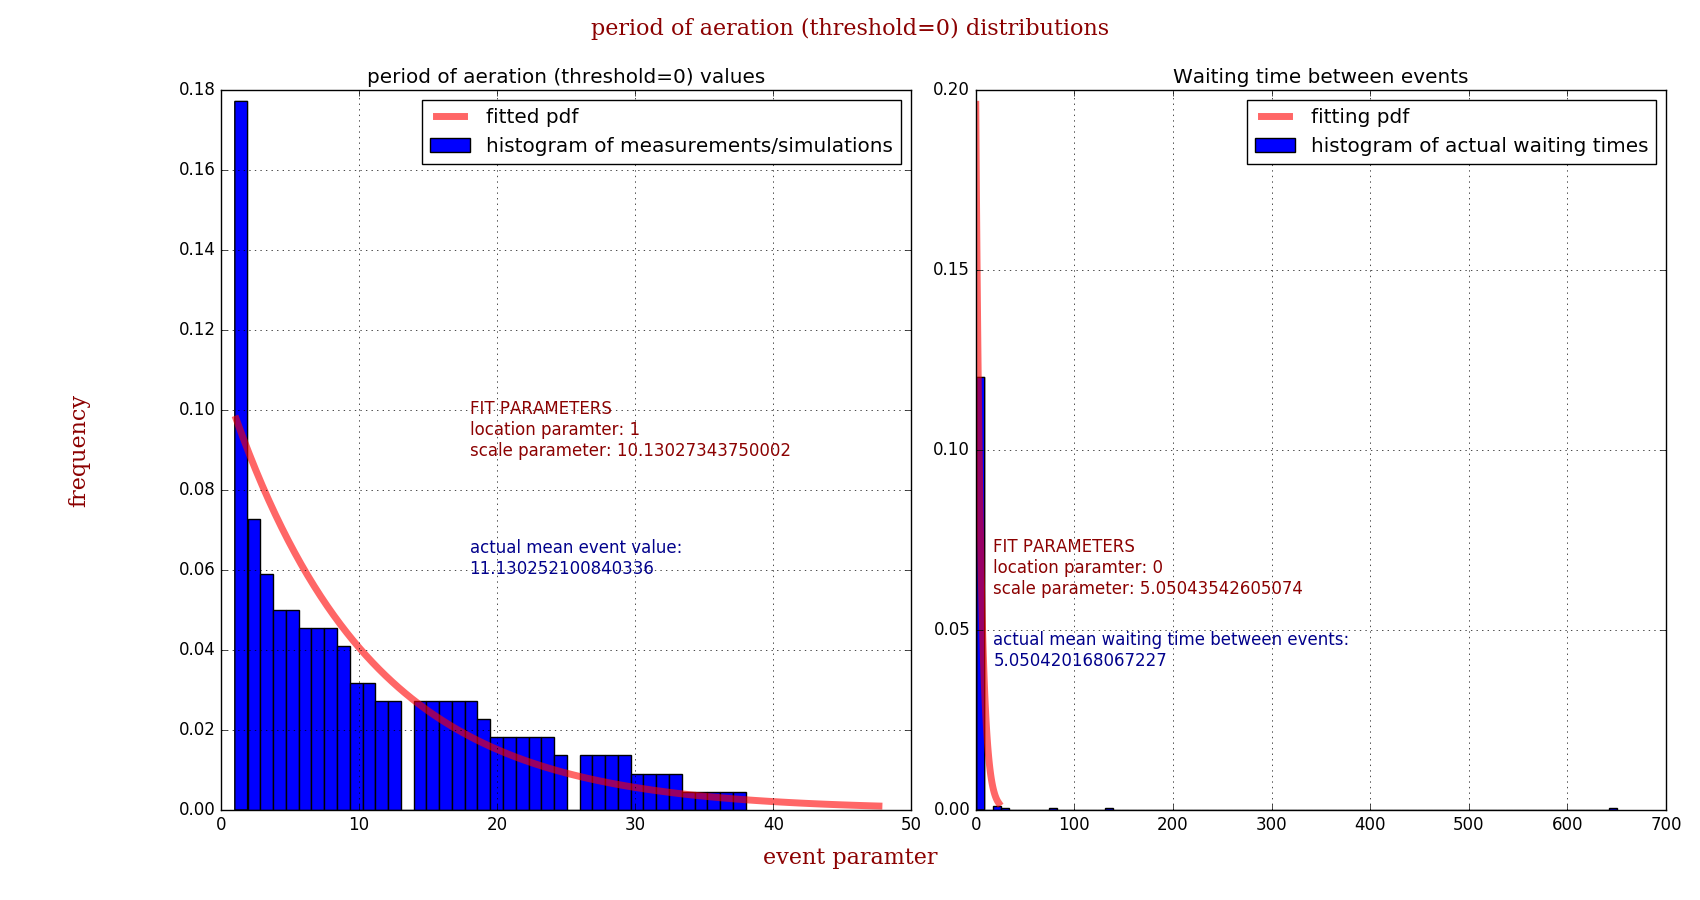
\includegraphics[width=\textwidth]{poa0}
\end{figure}
\begin{figure}[!htb]
\centering
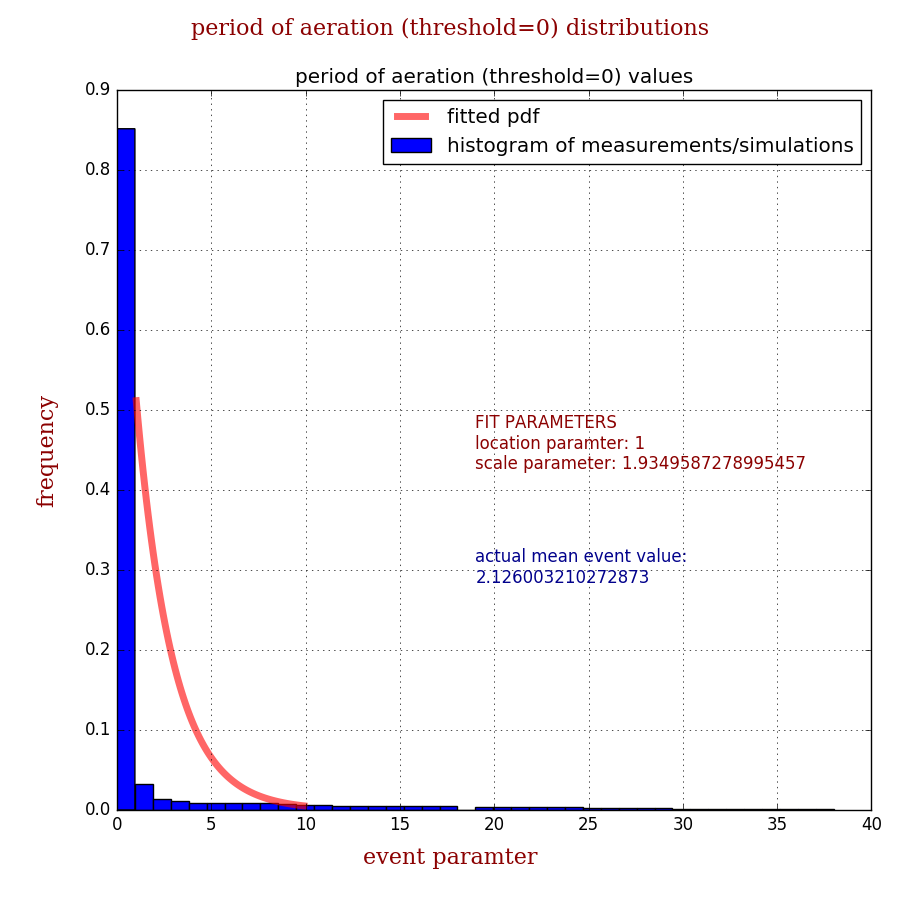
\includegraphics[width=.6\textwidth]{BULK_poa0}
\caption{Different behavior when 0 day periods allowed in histogram}
\end{figure}

\begin{figure}[!htb]
\centering
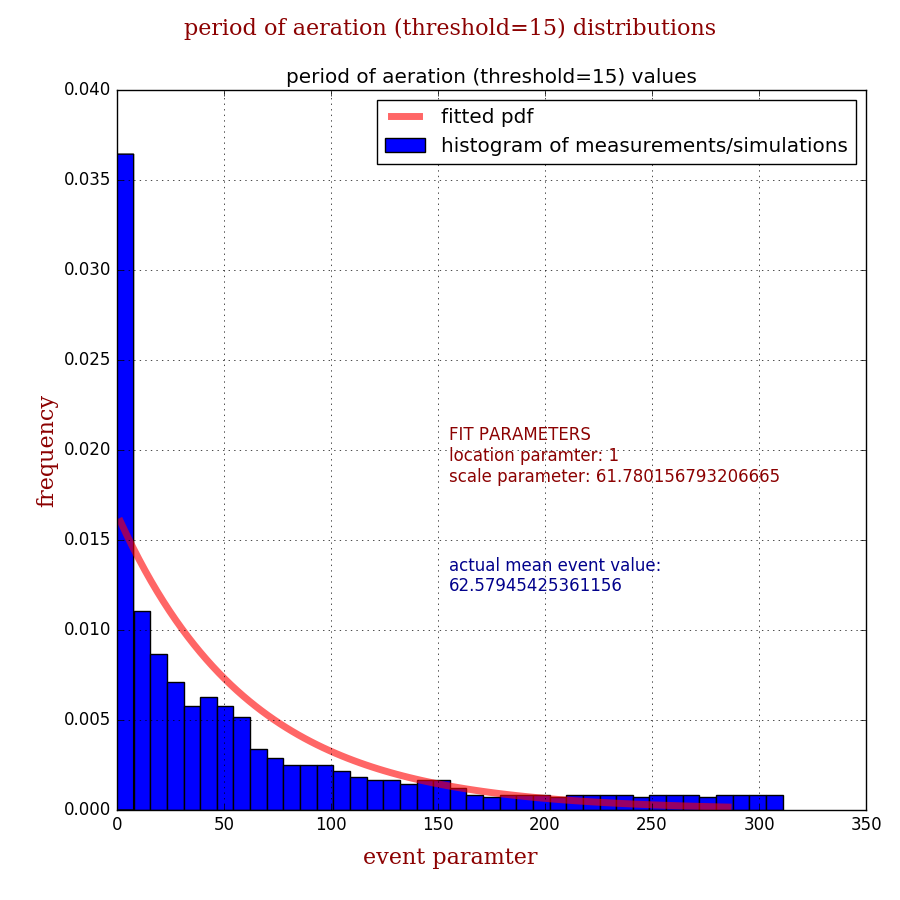
\includegraphics[width=.6\textwidth]{BULK_poa15}
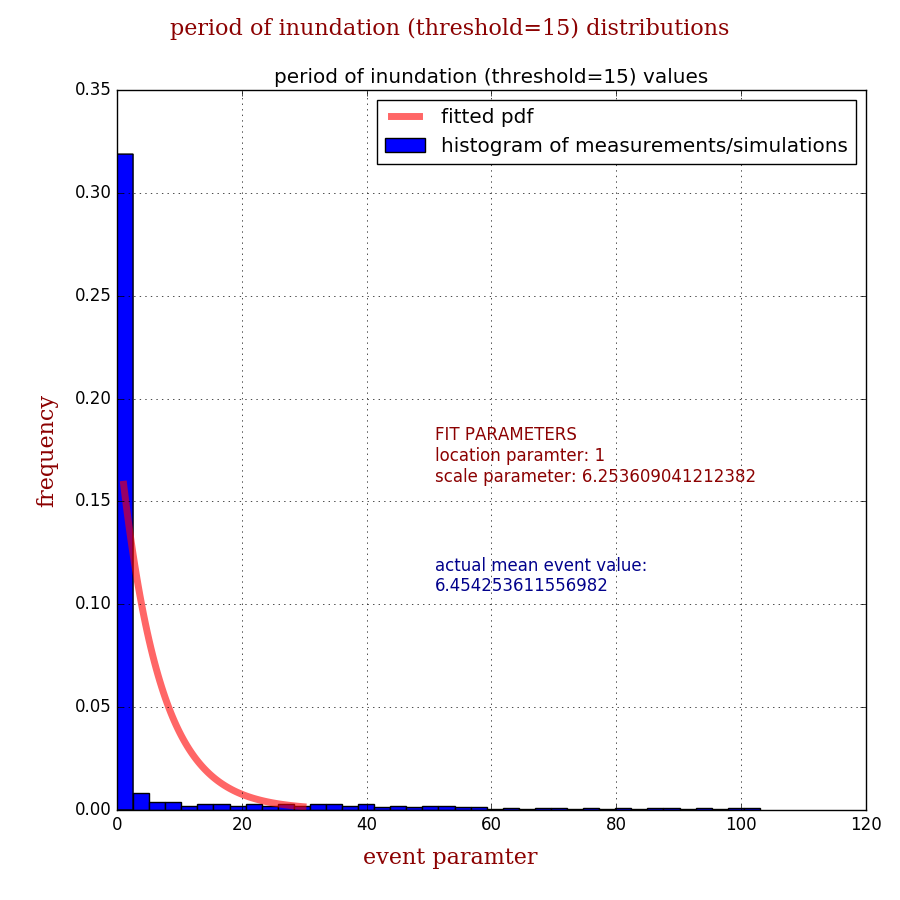
\includegraphics[width=.6\textwidth]{BULK_poi15}
\caption{Including 0 day periods results in good pdfs for either aeration or inundation sometimes, but never fits both well at the same threshold}
\end{figure}

\begin{figure}[!htb]
\centering
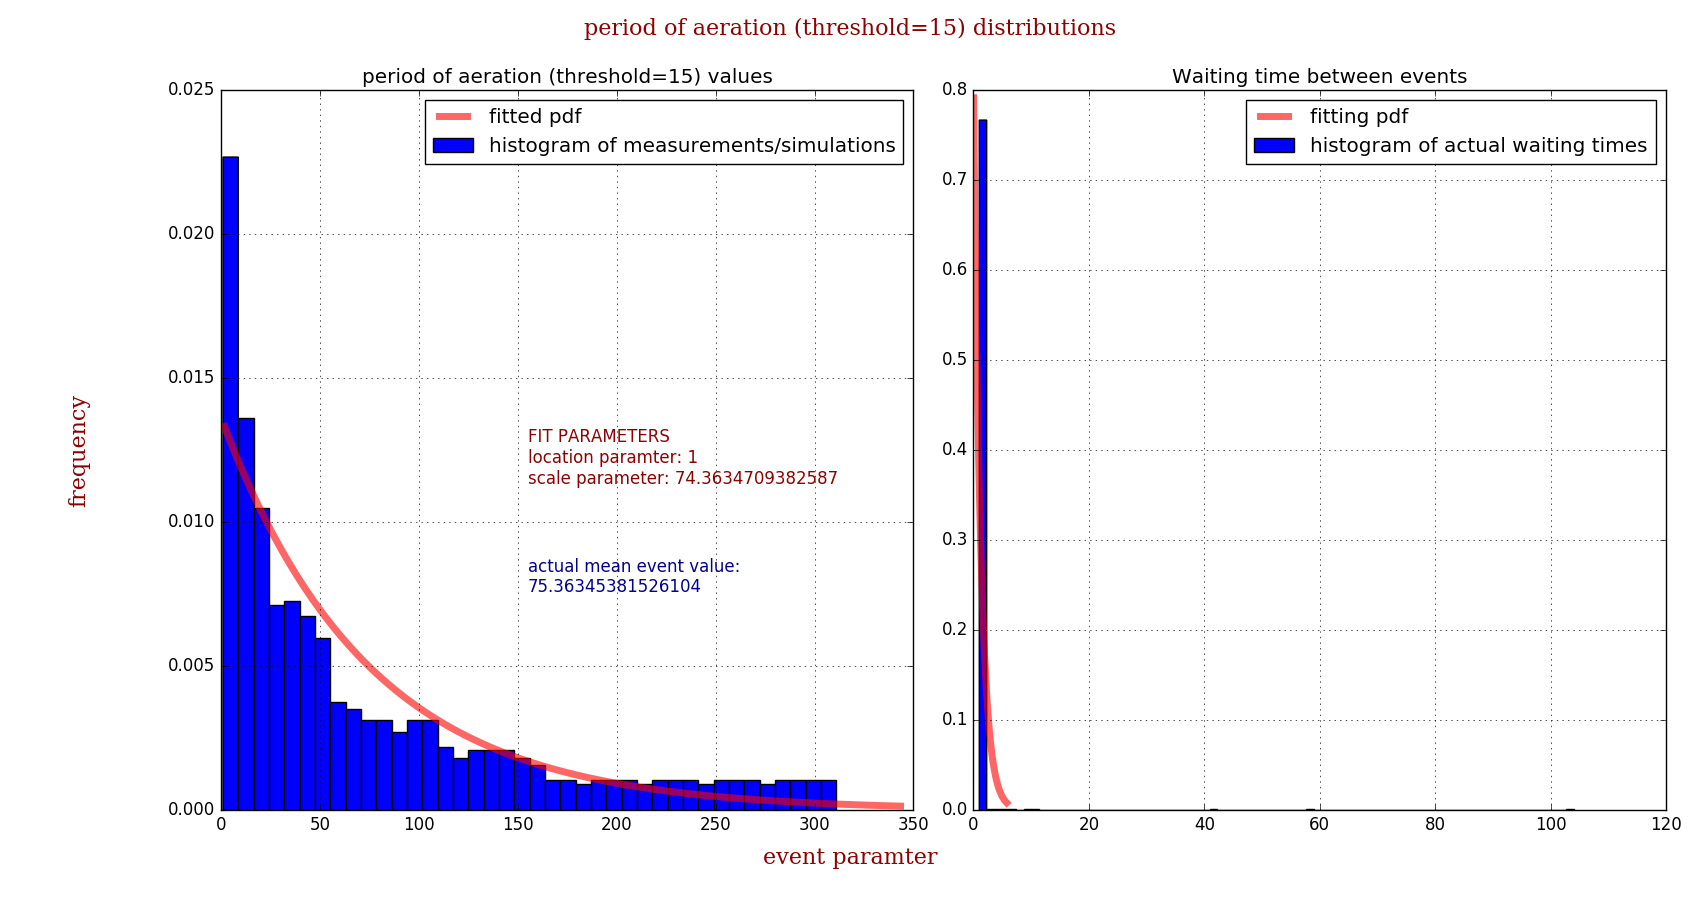
\includegraphics[width=\textwidth]{poa15}
\end{figure}
\begin{figure}[!htb]
\centering
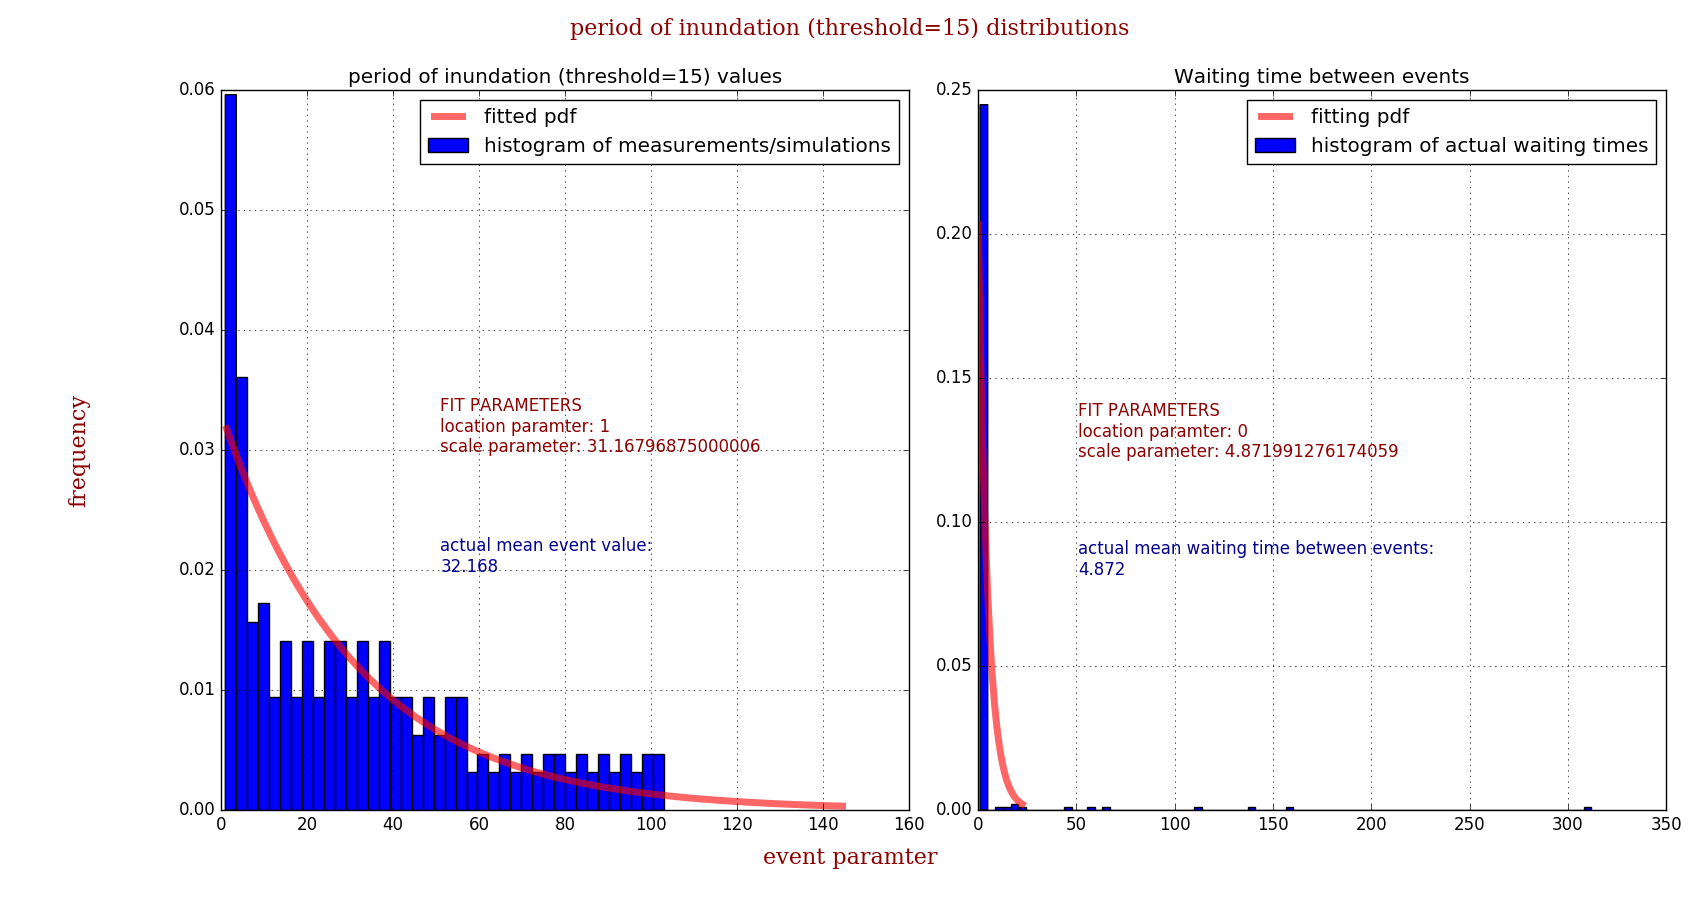
\includegraphics[width=\textwidth]{poi15}
\caption{Good fit at the same threshold when 0 day periods are removed. This is for threshold=15. See following pages for different thresholds.}
\end{figure}

\begin{figure}[!htb]
\centering
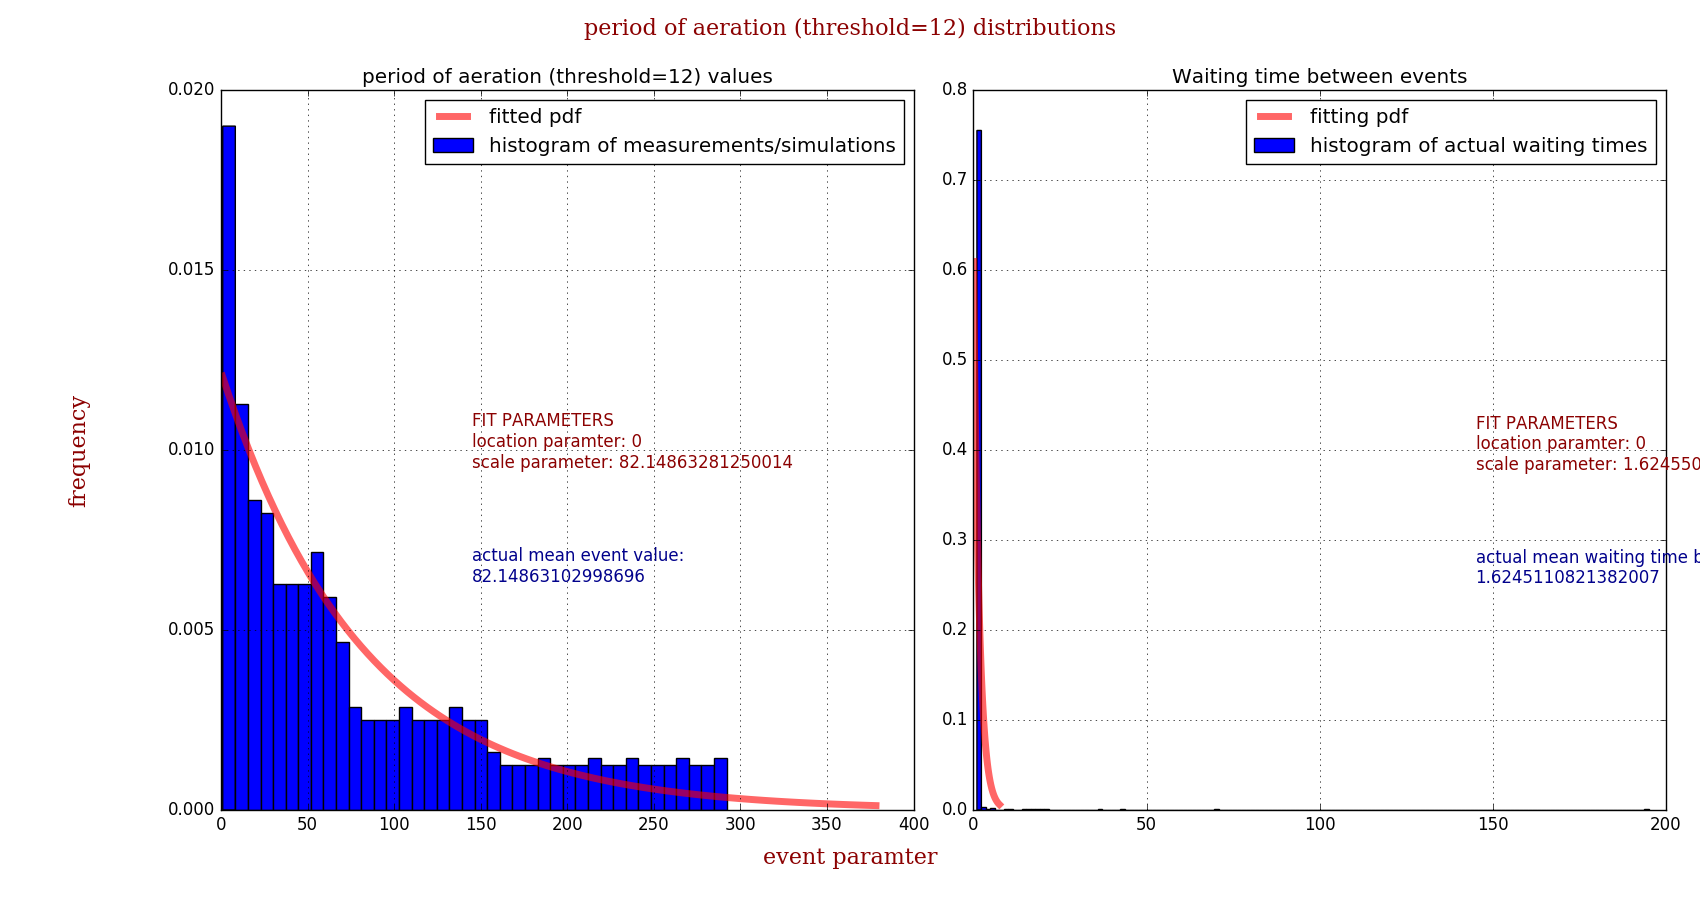
\includegraphics[width=\textwidth]{poa12}
\end{figure}
\begin{figure}[!htb]
\centering
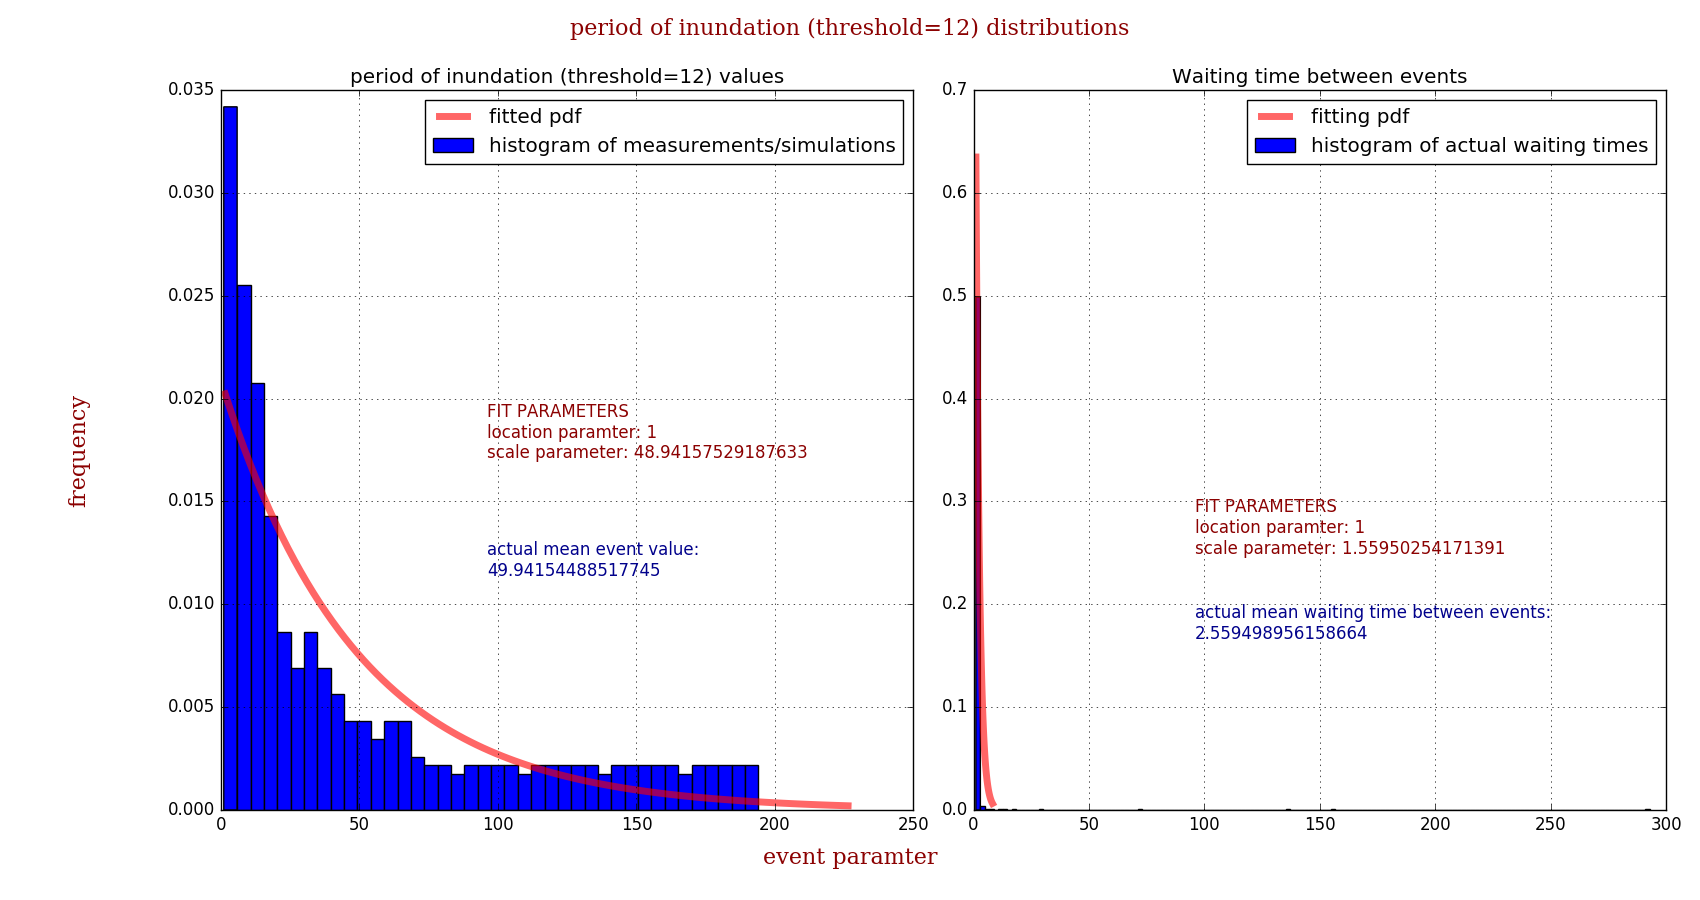
\includegraphics[width=\textwidth]{poi12}
\caption{Threshold=12.}
\end{figure}

\begin{figure}[!htb]
\centering
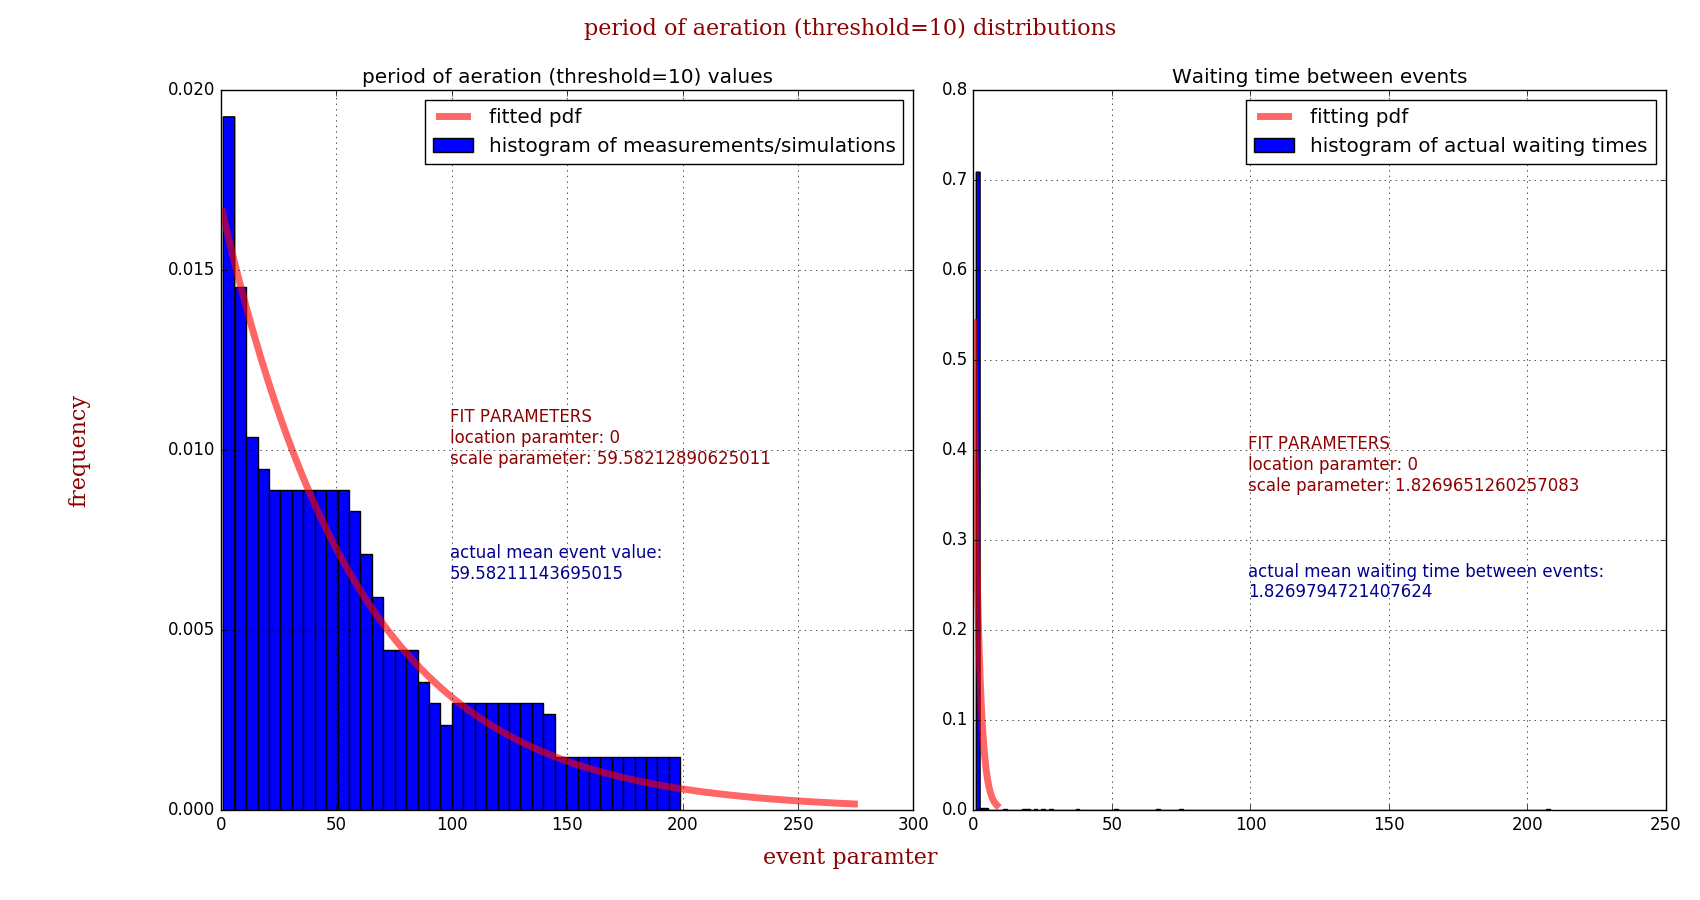
\includegraphics[width=\textwidth]{poa10}
\end{figure}
\begin{figure}[!htb]
\centering
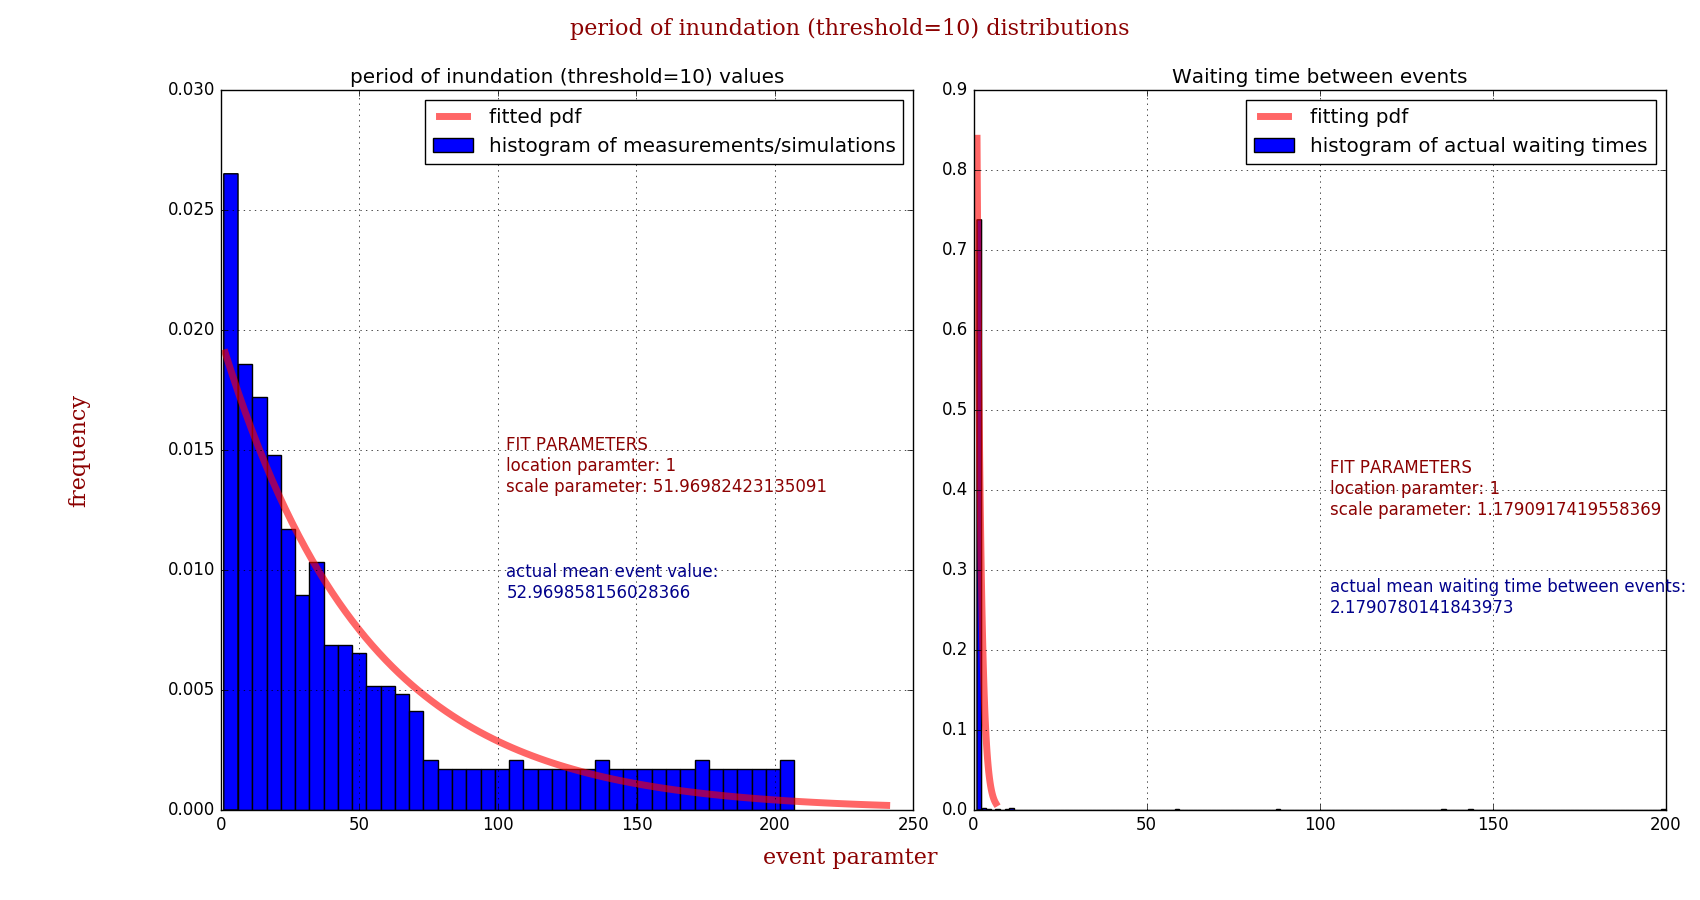
\includegraphics[width=\textwidth]{poi10}
\caption{Threshold=10.}
\end{figure}

\newpage
 In all of these, waiting time appears to be reasonably modeled by the exponential distrbution, and actually seems to be approaching the Dirac delta function. 






\end{document}